\documentclass{article}
\usepackage[utf8]{inputenc}
\usepackage{graphicx}
\usepackage{multicol}
\usepackage{framed}
\usepackage{float}
\usepackage{mathtools}
\usepackage{layout}
\author{Pedro Pereira, nº78889; Inês Roça, nº78164}
\usepackage{wrapfig}
\date{december 29, 2013}

%%Margens
\voffset=-3cm %%Posição apartir da vertical
\hoffset=-2cm
\evensidemargin=1pt
\textwidth=455pt
\textheight=700pt 


\begin{document}

%%Logotipo IST
\begin{wrapfigure}{l}{0.35\textwidth}
\vspace*{-3.5cm}
\hspace*{6.2cm}
    \includegraphics[width=0.35\textwidth]{tecnologico}
\end{wrapfigure}


%%Cabeçalho
\begin{flushright}
\begin{framed}
\begin{center} 
{\Huge\textbf{ O Microscópio}}
\vspace{.5cm}
\end{center}
{\large Trabalho final de Programação\\ Professor Samuel Eleutério\\Grupo 8 – 21/11/2013\\Pedro Pereira, nº78889;\\Inês Roça, nº78164}
\end{framed}
\end{flushright}

%%Documento em duas colunas

\begin{multicols}{2}
\section*{Microscópio Ótico Composto}

   O Microscópio é um instrumento de óptica composto por duas lentes delgadas\footnote{ Considera-se lente delgada toda a lente cuja espessura é significativamente menor do que o raio da curvatura, ou a distância focal.} convergentes – a objetiva e a ocular, que se encontram a uma determinada distância e que quando conjugadas permitem observar objetos de reduzidas dimensões e que se encontram muito próximos do sistema de lentes. Embora tenha sido instrumento imprescindível para o desenvolvimento da ciência, é um sistema bastante simples que tira partido das diversas propriedades das lentes utilizadas.

%%inserir imagem(nao resulta em 2 colunas)
%\begin{figure}[!htb]
%\begin{center}
%\scalebox{0.5}{\includegraphics{latex.jpg}}
%\caption{Diagrama de raios}
%%\end{center}
%\end{figure}

%%Inserir imagem numa de duas colunas
\begin{center}
\scalebox{0.6}{\includegraphics{olsss.jpg}}
\end{center}
\vskip -3mm\centerline{Diagrama de raios}
\vskip 2mm

Num microscópio, o objeto a observar é colocado pouco antes do ponto de foco da lente objetiva, formando-se uma imagem real e invertida do objeto. Assim a distância da imagem e do objeto pode ser relacionadas através da seguinte equação:
\begin{equation}
\frac{1}{d_{i}} + \frac{1}{d_{o}}=\frac{1}{f}
\end{equation}
\begin{flushright}
f- distância focal da lente;\\
d{\tiny i} - distância da lente à imagem;\\
d{\tiny o } - Distância do objeto à lente.\\
\end{flushright}

A ampliação da imagem obtida pela objetiva é assim:
\begin{equation}
M=\frac{-d_{i}}{d_{o}}
\end{equation}

\begin{flushright}
d{\tiny i} - distância da lente à imagem;\\
d{\tiny o } - Distância do objeto à lente.\\
\end{flushright}
 
A imagem formada pela objetiva corresponde ao objeto que será ampliado pela ocular, pelo que pode-se utilizar a equação (1) para relacionar as distâncias e a equação (2) para obter a ampliação da ocular.\\

Deste modo, a ampliação global do conjunto é dado pelo produto da ampliação de cada uma das lentes:


%%Equação numerada
\begin{equation}
M_{T}=\frac{-d'_{i}}{d'_{o}}.\frac{-d_{i}}{d_{o}}
\end{equation}
 
%% Fórmulas matemáticas sem numeração : \begin{displaymath}



\section*{Projeto}
\indent  Com o presente programa pretende-se simular virtualmente a ampliação de um determinado objeto pelo microscópio.\\ 

Assim, o utilizador dispõe de duas lentes delgadas convergentes, colocadas sobre um eixo horizontal, e cujas posições podem ser ajustadas quando pressionado o botão do rato sobre elas. Paralelamente às lentes e ainda sobre o mesmo eixo encontra-se um objeto cuja posição pode também ser adaptada devendo-se, no entanto, manter à esquerda do ponto de foco da lente objetiva.\\

Na janela surge ainda uma barra lateral, na qual é possivel selecionar a distância focal de cada uma das lentes bem como as dimensões do objeto em causa.\\

Selecionados os parâmetros desejados, o programa desenha o diagrama de raios de uma ampliação microscópica, tendo como base as relações estabelecidas nas equações (1), (2) e (3). Note-se que o programa permite que o utilizador opte pelos parâmetros que mais desejar, no entanto existem determinadas condições para que seja possível visualizar uma imagem ampliada num microscópio ótico.\\ \\

{\LARGE\textbf Situações Limite}

\begin{enumerate}

\item a distância focal da objetiva tem que ser sempre menor que a distância focal da ocular;
\item o objeto deve-se encontrar à esquerda do ponto de foco da objetiva, sem nunca o ultrapassar, pois para estas circunstâncias a imagem formada seria virtual, formando-se atrás da objetiva ; 
\item quando a ocular está na mesma posição que a primeira imagem, não é possível movimentá-la numa das direções para que o sistema de lentes não se comporte como o dado pela equação dos focos conjugados;
\item não é ainda possível posicionar os focos para fora do referencial

\end{enumerate}

\begin{center}
\scalebox{0.4}{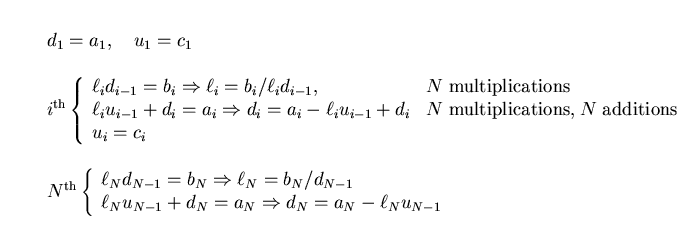
\includegraphics{2.jpg}}
\end{center}
\vskip -2mm\centerline{Limitação1}
\vskip 2mm


\begin{center}
\scalebox{0.38}{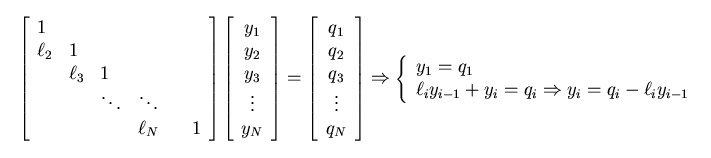
\includegraphics{3.jpg}}
\end{center}
\vskip -2mm\centerline{Limitação2}
\vskip 2mm

\begin{center}
\scalebox{0.4}{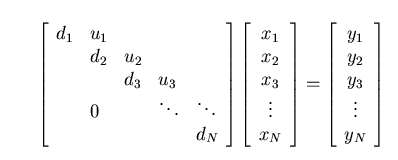
\includegraphics{4.jpg}}
\end{center}
\vskip -3mm\centerline{Limitação3}
\vskip 2mm


\begin{center}
\scalebox{0.4}{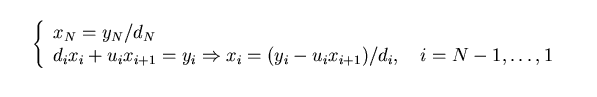
\includegraphics{5.jpg}}
\end{center}
\vskip -3mm\centerline{Limitação4}
\vskip 2mm

Estas limitações correspondem a condições necessárias para que o sistema se comporte como um microscópio, sendo portanto imprescindíveis para que o programa funcione de acordo com os objetivos.












\begin{thebibliography}{}

\bibitem{ma} D.Giancoli: 
\emph{Physics for scientists and engineers}, Pearson Prentice Hall, Upper Saddle River,4th edition.

\bibitem{ma} R, Serway e J, Jewett: 
\emph{Physics for scientists and engineers with Modern Physics}, Brooks/Cole, Belmont,8th edition.
\end{thebibliography}

\end{multicols}
\end{document}
